\section{Integrating threads}
\label{sec:babythreads}
After familiarising myself with the VSL codebase I tried to implement the simplest form of
multi-threading and test out how the language would behave. I added a new function to VSL
which takes a piece of code as an argument, starts a new thread and joins again with
the main thread. Once implemented, I could run the first and simplest unit test for ParVSL:

\begin{verbatim}
> (dotimes (i 4) (thread '(print "Hello World")))
"Hello World"
"Hello World"
"Value: Hello Worln"Hello Woird"
ld"
\end{verbatim}

We can immediately observe the effects of parallelism in action. The interpreter is not thread-safe and data races
on global variables (including printing to the same stream) lead to undefined behaviour. Printing
still seems to work, however most other functions would fail. The spawned threads can only handle strings
and will crash on handling numbers or symbols, or when trying to allocate anything.
There is no inter-thread communication, exception safety, and any garbage collection would produce a segmentation
fault. To be able to write a more complicated test, I need to make changes in all areas of the interpreter.

To manage the threads, I made further use of the C++11 standard library. I created a global hashmap storing
all the running threads. Creating and joining a thread is done under a mutex lock. Each thread is assigned its own unique
identifier, which is returned to the user. The user can then use the identifier to join the thread.

% \subsection{RAII classes}
% \label{sec:raii}
% The RAII (Resource Allocation Is Initialisation) design pattern is common in C++ \cite{effective-cpp}.
% It is a programming technique which binds the lifetime of resources to an object's lifetime. Normally,
% C and C++ are manually managed, meaning all resources have to be carefully tracked by the programmer.
% This makes it easy to introduce bugs when there is an attempted access to an unallocated resource,
% or leaks when a resource is not released after use. C++ classes offer a solution to this problem.
% Classes have both constructors and destructors, and these are automatically called when the object
% is created and when it becomes unavailable, respectively.

% \begin{verbatim}
% {
%   // obj1, obj2 are constructed here, unlike Java,
%   // where it would be a null reference.
%   Foo obj1;
%   Bar obj2;
% } // End of scope, obj2 is destructed, followed by obj1.
% Foo *obj3 = new Foo(); // Foo constructor called here.
% delete obj3; // Foo destructor is called here on obj3.
% \end{verbatim}

% We can use this mechanism to implement RAII. We simply make sure
% the underlying resource is allocated in the constructor and deallocated in the destructor.
% Smart pointers like \texttt{std::unique\_ptr} are a good showcase of the power of RAII. As soon as the
% smart pointer objects become inaccessible (e.g by going out of scope), the underlying pointer
% is safely deleted, providing a primitive (but very effective) form of automatic reference counting.

% When changing the codebase to use C++ features I found various opportunities to apply the RAII pattern,
% when managing threads, shallow binding and garbage collection.

% Thread objects in C++ are not implemented in a RAII style in the standard library. When a thread object
% is destructed, it must be in an \emph{unjoinable} state. A thread is unjoinable if it either has joined or
% it has been detached. If an unjoinable thread is ever destructed it will cause the entire C++ program to
% terminate.

% I have wrapped all threads in a \texttt{ThreadRAII} class, so that whenever they go out of scope they are automatically
% joined (when still in a joinable state). This guarantees there will be no premature termination in the case the
% user does not handle the thread correctly and that the ParVSL interpreter will exit cleanly.

% TODO: more robust code
% if there is an exception etc make sure it will always happen
% previous code spent time testing error flags

\section{Storage management}
\label{sec:storage}
All the memory is global and shared, and multiple threads will often try
to allocate concurrently, causing contention. A naive solution to this problem
would have been to use a mutex lock on allocations. While this would be easy to
implement, it would also severely degrade performance. Locks are expensive even
in single-threaded scenarios with no contention, and allocations are very common
when evaluating Lisp. This is especially the case in an interpreted Lisp where no
allocations are optimised away. Simply reading the code to evaluate allocates
\(O(n)\) times for code of length \(n\). That is because code in Lisp code is data.
Each instruction is a list data structure, with all elements allocated.
Serialising allocations is guaranteed to slow down the language enough to cancel
any advantage multi-threading brings to the language.

% \section{{\bfseries\sffamily TODO} Memory Allocation}
% Indeed, we can easily see the impact when trying to build reduce:

% \begin{center}
% \begin{tabular}{llll}
%  & VSL & MUTEX & SEGMENT\\
% \hline
%  &  &  & 2m1s\\
% \end{tabular}
% \end{center}


\subsection{Memory allocation}
\label{sec:malloc}
I wanted to allow multiple threads in parallel without affecting the performance
of allocations. To do this I had to use a lock-free approach. To do this, I further
split the memory into regions, which I call \emph{segments}. A segment is a thread-local region
for allocation in memory.

Just like before, memory is allocated to the segments in a continuous
fashion. A pointer indicates the start of the non-allocated part of the segment
(the \emph{segment fringe}.), while another tells us the end of the segment
(the \emph{segment limit}).

Now, contention is reduced to getting a new segment. Each thread only allocates within
its own segment, so allocations do not require any synchronisation, and they still only
require incrementing one variable in most cases. If the requested allocation would bring
the fringe over the segment limit, then the current segment is \emph{sealed} and a new one is
requested.

I carefully modified all the areas where allocations are preformed to use the segment fringe
instead of the global fringe. The global fringe is only moved to assign a new segment. Writes
to the global fringe are executed under a mutex lock, while the segment fringe is a thread local
variable accessed without any locks.

If the requested memory is larger than the segment size (e.g a large string or number),
the current segment is sealed, then the large object will occupy its own custom segment,
and the thread will then have to request a new segment.

There is a trade-off involved when choosing the segment size. If the size is too small,
there will be a lot of contention on requesting segments, leading back to the original
problem of locking on every allocation. If the segment size is too large, there is a risk
of threads holding large amounts of memory without using it and causing early garbage collection
cycles. This is because reclaiming memory is requested when a new segment cannot be created,
regardless of how much free space there is in existing segments. While the trade-off depends on the
total memory, I have found a good compromise for segments of a few kilobytes each.

\section{Garbage collection}
\label{sec:gc}
The \emph{garbage collector} (GC) has to account for the state of all threads. These threads have to be synchronised
and in a safe state to initiate the GC. They must also be included in the calculation of the root set.

I store all the thread-local information required for synchronisation in a class called \texttt{Thread\_data}. This
class is populated when a thread is started and updated before and after a GC cycle. All threads register
themselves in a global thread table at start-up. The thread starting the GC can use this table to check the status
of the other threads.

The \emph{ambiguous root set} is the set of potential references found on the stack. The stack is a continuous area
of memory managed by incrementing and decrementing a stack pointer. The stack pointer is normally not accessible
from C++, however we can take the address of a stack variable to find its location and hence approximate the
stack pointer's value. VSL remembers the position
of the stack at the beginning of the execution and calculates this again before garbage collection. Then it
scans the all locations in between for ambiguous roots.

\begin{verbatim}
uintptr_t C_stackbase;

int main() {
  // t is any variable on the stack, before execution of VSL code begins
  int t;

  // When starting VSL, we store the base of the stack
  // Here we need to cast the reference to an in type
  // then align to the size of a LispObject
  C_stackbase = ((intptr_t)&t & -sizeof(LispObject));
}

void garbage_collection() {
  int t;
  // before GC, we note the head of the stack
  uintptr_t C_stackhead = ((uintptr_t)&t & -sizeof(LispObject));

  // scan the stack from its head to base (the stack grows downwards)
  for (uintptr_t s = C_stackhead;
       s < C_stackbase;
       s += sizeof(LispObject))
  {
    if (in_heap(s)) { // check if s points within our virtual heap
      // we found an ambiguous root
      set_pinned(s);
    }
  }

  inner_garbage_collection();
}
\end{verbatim}

Each thread will have its own stack, so I had to modify the code to scan all the stacks before garbage
collection. This is one reason I had to pause work on all threads for GC. If I hadn't, then a thread might
add references to heap objects on its stack after those objects have been marked safe to delete, causing corruption.

When a thread is initialised, I save its own stackbase in \texttt{Thread\_data}, and then also save its stackhead
when it is paused to wait for GC. All these stack ranges are scanned before I start garbage collection:

\begin{verbatim}
void garbage_collection() {
  for (auto thread: thread_table) {
    // scan the stack from its head to base (the stack grows downwards)
    for (uintptr_t s = thread.C_stackhead;
         s < thread.C_stackbase;
         s += sizeof(LispObject))
    {
      if (in_heap(s)) { // check if s points within our virtual heap
        // we found an ambiguous root
        set_pinned(s);
      }
    }
  }

  inner_garbage_collection();
}
\end{verbatim}

% TODO: diagram
\subsection{Garbage collection locks and safety}
\label{sec:gclock}
The garbage collector is \emph{stop-the-world}. The thread initiating garbage collection must wait for all
threads to be ready. Similarly, all threads must regularly check whether a garbage collection cycle was
initiated and act accordingly.

The first idea I had was to trap all calls to allocate memory and check whether garbage collection is needed.
To do this, I could simply reset all thread segments. Threads would need to allocate eventually and
would request a new segment, at which point they would need to call the GC. This solution is incomplete however.
First of all, a thread might be busy for a long time without needing to allocate. This would cause all other
threads to be idle waiting for it to finish.

% TODO: deadlock diagram

A bigger issue was the risk of deadlocks. If thread A is waiting for the result of a computation on thread B,
but thread B was paused waiting for the GC, then the program is deadlocked. Similarly, any effectful computation,
like waiting for user input will prevent the collection from starting.

\begin{verbatim}
// global variables for synchronising garbage collection
std::atomic_int num_threads(0);
std::atomic_int safe_threads(0);
std::condition_variable gc_wait_all;
std::condition_variable gc_cv;
std::atomic_bool gc_on(false);
\end{verbatim}

To deal with the issue of blocking calls, I defined another state threads can be in: \emph{safe for GC}. A thread
is in a safe state if it has saved all the information the garbage collector needs to begin (e.g stackbase
and stackhead) and guarantees not to run any code that invalidates the garbage collection. Threads go into a safe
state whenever they get paused for GC. However, they can also be in safe state when waiting for a blocking call.

I created a special RAII class to handle both scenarios, which I called \texttt{Gc\_guard}. The class only has a constructor
and a destructor and is a way for the thread to promise it is in a safe state.

\begin{verbatim}
class Gc_guard {
public:
  Gc_guard() {
    int stack_var;
    // save the stackhead
    thread_data.C_stackhead =
      (LispObject *)((intptr_t)&stack_var & -sizeof(LispObject));
    paused_threads += 1;

    // notify the gc thread that this thread is in a safe state
    gc_wait_all.notify_one();
  }
   ~Gc_guard() {
    std::mutex m;
    std::unique_lock<std::mutex> lock(m);

    // wait here for gc to finish
    gc_cv.wait(lock, []() { return !gc_on; });
    paused_threads -= 1;

    // invalidate the stackhead
    thread_data.C_stackhead = nullptr;
  }
}
\end{verbatim}

The \texttt{Gc\_guard} class is accompanied by \texttt{Gc\_lock}. A thread trying to initiate the GC will have to
acquire a \texttt{Gc\_lock}. The lock will wait until all threads are in a safe state and will prevent
other threads from acquiring.

% TODO: fix this code
\begin{verbatim}
class Gc_lock {
  std::mutex m;
  std::unique_lock<std::mutex> lock;
  Gc_guard gc_guard;
public:
  Gc_lock() : m(), lock(m) {
    int stack_var = 0;
    thread_data.C_stackhead =
      (LispObject *)((intptr_t)&stack_var & -sizeof(LispObject));

    paused_threads += 1;
    gc_wait_all.wait(lock, []() {
      return paused_threads == num_threads;
    });
  }

  ~Gc_lock() {
    paused_threads -= 1;
    gc_on = false;
    thread_data.C_stackhead = nullptr;
    gc_cv.notify_all();
  }
};
\end{verbatim}

% \section{{\bfseries\sffamily TODO} just having a non-stop gc would be its own project}
% \label{sec:org55eb9ba}
% reference java, etc. but what I have is good enough
% interlocks add overhead, but w do not need real-time performance
% not many threads

\section{Lock-free hashtable for symbol lookup}
\label{sec:hashtable}
Just like allocations are a critical region of code in VSL, so are symbol lookups.
Every occurrence of a symbol must be looked up in the symbol table. If the symbol does
not exist, it will be created. Multiple threads looking up symbols will cause contention.
If two threads try to allocate the same symbol name at the same time, they will invalidate
the table.

As before, the naive solution would be to implement a mutex lock on the entire
lookup function.

To improve on that I tried to use a reader-writer lock. Reader-writer locks allow grant access
to either a single writing thread, or all the reading threads. This would would allow multiple
threads to lookup symbols at the same time, however, as soon as one one thread has to create a
symbol, all the readers have to wait for it to finish.

Moreover, the lookup function is two-step: first it tries to find a symbol, then it creates one
if it didn't find any. If two threads lookup the same symbol at the same time, it is possible for
both of them to end try to create it at the same time. The reader-writer lock would not prevent this!
It would serialise the writes, so it does prevent undefined behaviour in C++, however it does still
create the symbol twice. The pointer to the symbol that the first thread returned from the function
would become invalid.

I have found a third approach, based on the Compare-And-Swap (CAS) instruction which solves the issue
above, while also providing a lock-free implementation. The symbol lookup table is currently implemented
as a static array of linked lists. VSL never erases symbols, which made the lock-free implementation easier.

\begin{figure}
\begin{verbatim}
std::atomic<LispObject> symbol_table[TABLE_SIZE];

LispObject lookup(std::string name) {
  size_t loc = hash(name) % SYMBOLS_SIZE;

  LispObject bucket = symbols[loc].load(std::memory_order_acquire);

  while (bucket != nil) {
    LispObject s = head(bucket); // first list element

    if (symbol_name(s) == name) {
      // found the symbol
      return s;
    }

    bucket = tail(bucket); // rest of the list
  }

  LispObject s = allocate_symbol(name);

  LispObject new_bucket = cons(s, bucket);

  while (!symbols[loc].compare_exchange_strong(
      bucket, new_bucket, std::memory_order_acquire_release))
  {
    // search for stored value
    LispObject old_bucket = bucket;
    bucket = symbols[loc].load(std::memory_order_acquire);

    for (LispObject s; s != old_bucket; s = tail(s)) {
      if (symbol_name(s) == name) {
        // Another thread created the symbol. Use that.
        return s;
      }
    }

    // Make sure we don't discard new symbols inserted by other threads.
    new_bucket = cons(s, bucket);
  }

  return s;
}
\end{verbatim}
\caption{Lock-free symbol hashtable look up implementation}
\label{code:lockfree}
\end{figure}

This approach adds no penalty to single-threaded
code. For comparison, I also implemented the mutex lock approach and tested
them on building Reduce (single-threaded). Table \ref{fig:lockfree} shows that the mutex
version is noticeably slower.

\begin{figure}
  \centering
  \begin{tabular}{lr}
                               & Time \\
  \hline
  VSL                          & 1m55s \\
  ParVSL with mutex lookup     & 2m10s \\
  ParVSL with lock-free lookup & 1m55s \\
  ParVSL with std::string      & 2m04s
  \end{tabular}
  \label{fig:lockfree}
  \caption{Symbol lookup effects on building Reduce}
\end{figure}

\subsection{Impact of C++ \texttt{std::string} on performance}

While modifying this code, I saw the opportunity to change C-style string to C++
standard library ones. The lookup function, for example, actually takes a char array
pointer and the string length as separate arguments. I even identified a bug
in VSL where the wrong length was passed as a hard-coded number, and it prompted
me to use the more modern \verb|std::string| class. To my surprise, this change alone
slowed down ParVSL, as can be seen in the last row of Table \ref{fig:lockfree}.
I made sure no more extra copying or construction of these strings was done than
necessary. I reverted my change in this case, but I note it as an interesting example
of the trade-off C++ features can bring.

% times
% vsl 0m14.353s
%     0m13.764s

\section{Symbol access}
\label{sec:symbols}
\label{sec:datarace}
The interpreter is the core of VSL. It runs a read-eval-print loop which makes heavy use of global state and side effects.

All named objects in the lifecycle of the program are \emph{symbols}. All global and local variables, including
special ones (like \texttt{true} or \texttt{nil}) and function arguments are symbols. A global hash-table keeps track of
all symbols. This means each name can only be in use in one place at a time.

Lisp is a language with dynamic scope. This has many implications for the interpreter. The following
fragment of code is an example of this behaviour:
\begin{verbatim}
let f x = x + y in
let g () =
  let y = 3 in
  f 2
in
g ()
\end{verbatim}

The above example will not compile in any statically scoped languages such as OCaml or C++
because the variable \texttt{y} is not defined in its scope.
Most dynamic languages, even weakly typed ones, like Javascript or Python, will allow equivalent
code as valid, but will encounter a runtime error because \texttt{y} is not defined.
Lisp, and VSL in particular, has a mach looser concept of scope.
In the example above, \texttt{y} is defined before the call of \texttt{f} and will remain defined until the
call to \texttt{g} returns.

\emph{Shallow binding} is the mechanism by which this is achieved. Each symbol is mapped to a single value.
When a variable name is bound, e.g. as a function parameter name during a function call or through a
\texttt{let} statement, its old value is stored by the interpreter and replaced with the new value. At the end of the binding,
the old value is restored. The main advantage of this method is performance. Old values can simply be saved
on the stack:
\begin{verbatim}
let varName = expr1 in expr2
\end{verbatim}

can be implemented as:

\begin{verbatim}
void implement_let(string varName, LispObject expr1, LispObject expr2) {
  LispObject symbol = lookup_symbol(varName);
  LispObject oldVal = value(symbol); // store the old value
  value(symbol) = eval(expr1);       // replace with new value
  eval(expr2);                       // evaluate the rest of the code
  value(symbol) = oldVal;            // restore old value
}
\end{verbatim}

This mechanism was not designed with concurrency in mind, and is not thread-safe.
Many variable names are reused multiple times in a program (e.g \texttt{i, j, count}, etc).
Multiple threads binding the same variable will override each other's values.

I wanted to fix this while keeping the same dynamic scoping semantics for backward compatibility.
One option was implement a form of deep binding with functional association lists storing local values,
however I was concerned with the performance. Shallow binding has a constant factor, while any
associative data structure would add non-negligible overheads to a critical area of the
interpreter (symbol lookup).

My approach was to allocate thread-local storage for symbols.
Global symbols were unaffected, because rebinding them is illegal in the language.
However, for non-globals I used a thread-local array to store the real value, and had the global storage
location point to the array location. Each local symbol gets its own unique array index for the lifecycle
of the program. Then, each thread will reserve that location within its local array for the symbol.

\begin{verbatim}
thread_local vector locals;
vector shared_fluids;

LispObject par_value(LispObject symbol) {
  // [value] returns the symbol's global value
  LispObject val = value(symbol);

  if (is_global(symbol))
    return val; // global symbols remain unaffected

  int loc = to_int(val); // val is a location

  if (is_fluid(symbol) and locals[loc] == undefined)
    // No local value for this fluid. Return the global one.
    return shared_fluids[loc];

  // get the thread-local value at that location
  return locals[loc];
}
\end{verbatim}

I carefully replaced all calls to \texttt{value} to \texttt{par\_value}. Now, multiple threads accessing the same symbol
can do so safely, as they will each access their own versions. This eliminates data races entirely,
and shallow binding is unaffected.

\begin{figure}[H]
  \centering
  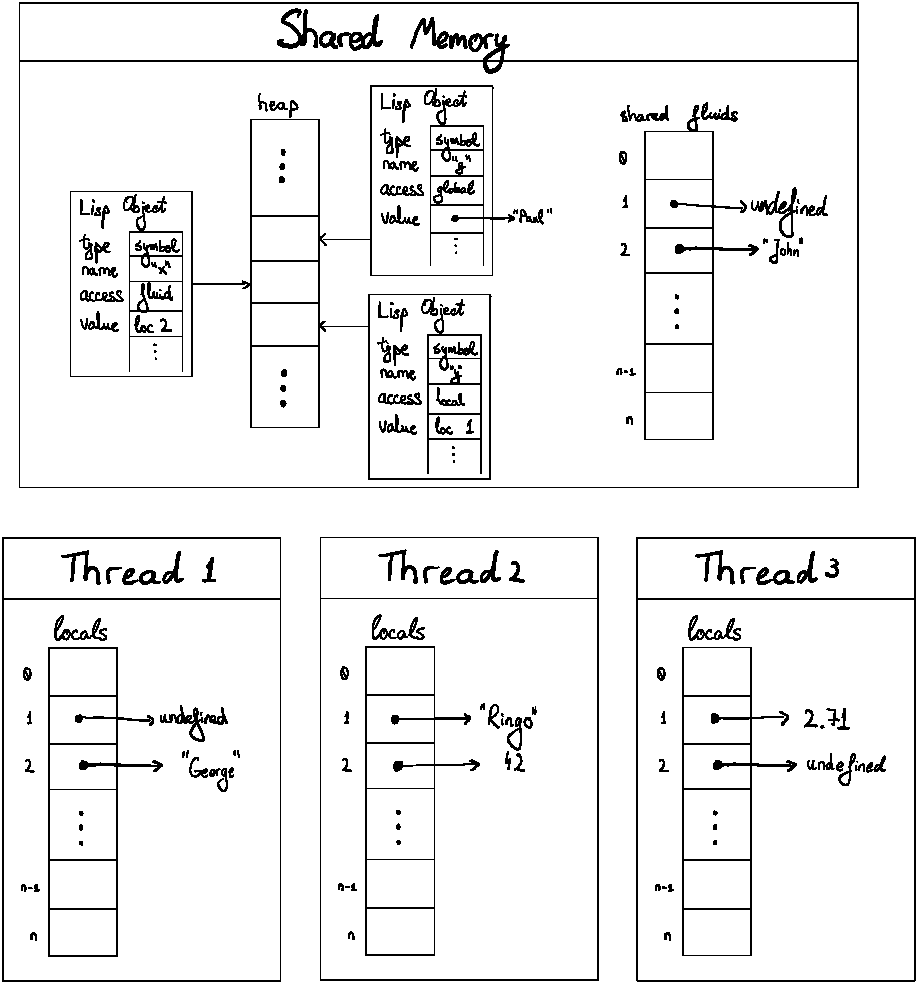
\includegraphics[width=1\linewidth]{symbols.pdf}
  \label{fig:symbols}
  \caption{Storage of symbols in ParVSL}
\end{figure}

In figure \ref{fig:symbols} I show a full example of how symbols are stored. The first symbol is \texttt{g}, which
is a \emph{global} symbol. It's value is stored directly in the global heap (like in the original VSL). The symbol \texttt{x}
is \emph{fluid}. It's heap value simply indicates a location (\texttt{loc 2}). We use the index to find the actual value
in thread-local storage. Threads 1 stores the string \texttt{"George"} while thread 2 stores the integer \texttt{42}.
Thread 3 has not bound any local value to the symbol so it is \texttt{undefined}. However, it can still access the
global value in \verb|shared_fluids|, the string \verb|"John"|. Finally, symbol \verb|y| is \emph{local}. It is
undefined in \verb|shared_fluids| but otherwise behaves the same as \verb|x|, storing its thread-local values at
index \verb|1|.

% \begin{center}
% \begin{tabular}{llll}
%  & VSL & MUTEX & LOCK-free\\
% \hline
%  & 1m55s & 2m10s & 2m4s\\
% \end{tabular}
% \end{center}

\section{Threads}
\label{sec:threads}

To start a thread, the user
simply needs to call the \texttt{thread} function. This function takes as arguments a function name and the argument list
and a unique thread id is returned. The function is applied to the arguments in a new thread. The return value
is stored until the user call \texttt{thread\_join} on the thread id, when they can access the respective value.

\begin{verbatim}
tid := thread('add, {2, 3});
result := thread_join tid;
print result;
\end{verbatim}

This allows for simple inter-thread communication, through function parameters and returns. Any function can
be run in parallel by simply applying thread on it. This task based approach makes it easy to modify
single-threaded algorithms to run in parallel.

My implementation minimises overhead. The list of arguments is managed on the heap which is visible by all
threads, so a simple pointer is enough to pass them. For returning values, I must keep track of all
unjoined threads and their return values. I do this with a simple hashtable, mapping thread ids to their
return values. When a thread returns from its function, I update the hashtable with the returned value.
When the user joins a thread, I look up the value in the table, return it, then erase the mapping. All threads
have unique ids for the lifetime of the program, so there will never be conflicts in the hashtable.
This hashtable has to be thread-safe, and I have implemented it as described in Lock-free hashtable.

I must also be careful to prevent the garbage collector from collecting these parameters and return values.
Starting a thread is GC-safe: garbage collection will not begin while a new thread is starting up. This ensures
that threads are always in a safe state and registered in the thread-table correctly during garbage collection.
At that point, function parameters are tracked just like regular variables so they will be safe from GC.
However, return values are stored past the lifetime of their respective threads. To deal with them, I add them
to the root set at the beginning of garbage collection.

The handling of both of these root sets has to account for multiple running threads. All the new
thread-local storage was added to the unambiguous root set. Additionally, each thread is running its
own stack so all the stacks has to be accounted for as the ambiguous root set. The latter is more complicated.
All threads have to be paused before garbage collection can begin so that they do not interfere
with memory. A simple way to do this is to enable a global flag which all threads check on a regular basis.
However, if we are not careful, this can easily cause a deadlock (e.g: thread A waits for a signal from
thread B, but thread B is waiting for garbage collection). To solve such issues, I need to make two
changes. First, I must modify the functions in the interpreter to poll the global flag. Then I have
to make all waiting calls put a thread into a \emph{safe} state before sleeping, so that the garbage collector
can proceed with the thread.

\section{Saving state to disk and reloading}
\label{sec:preserve}

One important feature of the language is the ability to preserve the state of the world at any
time and save to disk. It is difficult to keep the same guarantees when multiple threads are running:
preserving when some of the threads are running a computation is tricky to define properly. To simplify
matter, I have decided that all threads have to be joined before preserving. This way, the state of
the world is consistent and relatively easy to restore. I have modified parts of the code to write
all the thread-local data back into global storage and then restore it when reloading. This way the same
file format is preserved, and I have not broken compatibility between single and multi-threaded images.

Implementing ParVSL, I introduced additional state and book-keeping to manage the extra complexity.
When preserving in VSL, all this state is stored to a file by compressing a bit for bit copy of the
content. The main use for this is saving the results of computations and function definitions.
The REDUCE build is stored in the same way. After building all the necessary files,
it preserves the current state inside an image. Loading the image on startup of VSL will effectively
start REDUCE.

I wanted to keep the VSL image format in ParVSL so that I would not break compatibility between the two.
I note that preserving a running multi-threaded program would be impossible without making major changes
to the image format and major redesign of the code. Calling \texttt{preserve} also stops the pr

 If a thread attempts to preserve while others
are running, the contents of the final image would be non-deterministic and generally undesirable,
even if I were to resolve all data races. At the same time, I found little benefit to implementing such
a feature, as the ability to preserve is useful to retain results of computations, not intermediate states.
Saving state to disk is an operation happening at the end of the program.

My implementation on preserve preservation only allows the operation on the main thread, and will wait
for all spawned threads to finish running and join.